\documentclass[journal]{IEEEtran}
\IEEEoverridecommandlockouts

\usepackage{amsmath,amssymb,amsfonts}
\usepackage{graphicx}
\usepackage{booktabs}
\usepackage{url}
\usepackage{xcolor}

\newcommand{\todo}[1]{\textcolor{red}{\textbf{[TODO: #1]}}}

\DeclareMathOperator{\rank}{rank}
\DeclareMathOperator{\range}{range}
\newcommand{\bG}{\mathbf{G}}
\newcommand{\bS}{\mathbf{S}}
\newcommand{\bB}{\mathbf{B}}
\newcommand{\bW}{\mathbf{W}}
\newcommand{\bZ}{\mathbf{Z}}
\newcommand{\bJ}{\mathbf{J}}
\newcommand{\bD}{\mathbf{D}}
\newcommand{\bU}{\mathbf{U}}
\newcommand{\bg}{\mathbf{g}}
\newcommand{\CN}{\mathcal{CN}}
\newcommand{\Hank}{\mathcal{H}}
\newcommand{\reff}{r_{\mathrm{eff}}}
\newcommand{\rmax}{r_{\max}}
\newcommand{\dhs}{\Delta_{\mathrm{HS}}}

\begin{document}

\title{Hankel-Structured Channel Estimation for Rydberg\\
Atomic Receivers: Bounds, Effective-Rank Scaling,\\
and Out-of-Model Validation}

\author{Abdullah~Haatim%
\thanks{A.~Haatim is with the \todo{CONFIRM DEPARTMENT: this string is the one
used in the earlier HS-GS draft of this project; it is not an independent
source} Department of Electrical and Electronics Engineering, Birla Institute
of Technology and Science, Pilani~--- Pilani Campus, India (e-mail:
f20220519@pilani.bits-pilani.ac.in).}}

\maketitle

\begin{abstract}
Rydberg atomic receivers measure field magnitude only, making multi-user
channel estimation a biased phase-retrieval problem in which unstructured
solvers are flat in array size: their Fisher information is block diagonal
across receive elements, so a larger aperture buys nothing under a normalised
metric, and only a structural prior converts aperture into accuracy. We
enforce the low-rank Hankel structure of the uniform-linear-array response
inside an exact expectation--maximization Gerchberg--Saxton iteration, select
the order from a held-out pilot residual, and benchmark against a Rician
Cram\'er--Rao bound in which each magnitude measurement contributes rank-one
information, together with a geometry-constrained bound on the
$3\sum_k L_k$-parameter manifold. The gain grows from $+0.03$ to $+2.45$~dB as
$N$ goes $8\to32$ while the unstructured baseline moves by $0.036$~dB. We then
show the governing variable is not path count but effective rank relative to
capacity, and use that relation to predict the gain on two channel models it
was never fitted to. Simulation only; the bounds do not govern biased
estimators.
\end{abstract}

\begin{IEEEkeywords}
Rydberg atomic receiver, channel estimation, phase retrieval, Hankel matrix,
constrained Cram\'er--Rao bound, effective rank.
\end{IEEEkeywords}

\section{Introduction}

\IEEEPARstart{A}{tomic} receivers based on Rydberg states read out radio fields
through an optical transition whose response is proportional to field
\emph{magnitude}, discarding phase~\cite{cui2025,gong2025mag}. Multi-user
channel estimation is therefore biased phase retrieval, and
Gerchberg--Saxton-type alternating projection~\cite{gerchberg1972} is the
natural solver; recent work unrolls it into a trained
network~\cite{xiao2026}, and a rank projection has been placed inside
projected gradient descent for the same problem~\cite{xu2025}.

Unstructured solvers share a limitation that is easy to miss and, once seen,
explains a great deal: \textbf{their accuracy does not improve as the array
grows.}
Row $n$ of $\bG\bS$ enters only measurement row $n$, so the Fisher information
is block diagonal across receive elements and the per-element estimation
problem is unchanged by adding elements. Aperture is only useful to an
estimator that couples elements --- which is exactly what a structural prior
does.

On a uniform linear array (ULA) each propagation path contributes one spatial
complex exponential, so the Hankel lifting of every channel column is rank
deficient~\cite{cadzow1988,markovsky2008}. Enforcing that inside the iteration
turns aperture into accuracy. But knowing \emph{when} it applies has, until
now, meant a qualitative appeal to sparsity, and that is unusable: a $16$-path
channel on a $32$-element array is algebraically full rank yet has effective
rank $8.73$, and its lifting is compressible with nothing sparse about it.

\textbf{Contributions.}
\begin{enumerate}
\item A benchmark, not just a baseline: a Rician Cram\'er--Rao bound in which
each magnitude measurement contributes \emph{rank-one} information, and a
geometry-constrained bound in tangent-space form because the parameterisation
is rank deficient. EM-GS sits within $0.05$~dB of the unconstrained bound, so
the benchmark is credible.
\item The aperture-scaling result and its Fisher-information explanation.
\item Replacement of the path-count heuristic by $\reff/\rmax$, with the
capacity $\rmax=\lceil N/2\rceil$ derived.
\item Two out-of-model predictions, each registered before measurement, on
channel models the relation was never fitted to --- the clustered-propagation
falsification test that this work's earlier stage identified as decisive.
\end{enumerate}

\section{System Model}

An $N$-element ULA serves $K$ single-antenna users over $P$ pilots. With
$\bG\in\mathbb{C}^{N\times K}$, pilots $\bS$, known reference beam $\bB$ and
noise $\bW$, the receiver observes
\begin{equation}
\bZ=\left|\bG\bS+\bB+\bW\right|,\qquad \bW_{np}\sim\CN(0,\sigma^2),
\label{eq:obs}
\end{equation}
elementwise, and the modulus is never linearised. User $k$'s channel is
\begin{equation}
\bg_k=\sum_{\ell=1}^{L_k}\alpha_{k\ell}\,\mathbf{a}(\theta_{k\ell}),\qquad
[\mathbf{a}(\theta)]_n=e^{-j\pi n\sin\theta},
\label{eq:chan}
\end{equation}
so each column is a sum of complex exponentials in the element index.

\textbf{RSR convention, stated once.} The reference-to-signal ratio is defined
against a \emph{single} user. Since $K$ users transmit at once, a nominal
single-user RSR of $12$~dB is $12-10\log_{10}K=7.23$~dB against the $K$-user
total at $K=3$; $10$~dB single-user is $5.23$~dB.~\todo{An earlier draft of
this work stated $7.15$~dB for the $12$~dB case; the arithmetic gives $7.23$~dB
and the $0.08$~dB difference could not be reconciled from any stored result.
Confirm which is intended.} All RSR values quoted here are single-user.

\textbf{Two averaging domains, kept distinct.} Within an operating point NMSE
is pooled as a ratio of sums,
\begin{equation}
\mathrm{NMSE}=10\log_{10}\frac{\sum_t\|\hat\bG_t-\bG_t\|_F^2}
{\sum_t\|\bG_t\|_F^2},
\label{eq:nmse}
\end{equation}
never a mean of per-trial decibels: \eqref{eq:nmse} estimates the ensemble
quantity a Cram\'er--Rao bound bounds, whereas a mean-of-decibels is smaller by
Jensen. Across SNR, the mean is of per-SNR decibel values, after conversion;
linear NMSE spans three orders of magnitude, so a linear average across SNR is
dominated by the lowest-SNR point and nearly blind to the high-SNR half.
\textbf{Rule used throughout:} ratio-of-sums wherever a curve is compared to a
bound; paired per-trial median with a bootstrap interval for paired contrasts.
Both are reported; neither is used for the other's job.

\section{Hankel Structure and the HS-GS Estimator}
\label{sec:method}

For $\bg\in\mathbb{C}^N$ and pencil $p$, let $\Hank_p(\bg)$ be the
$(N-p)\times(p+1)$ Hankel matrix. Under \eqref{eq:chan} its rank is
$\min(L_k,N-p,p+1)$, so the largest expressible rank is
\begin{equation}
\rmax(N)=\max_{p}\min(N-p,\,p+1)=\left\lceil N/2\right\rceil,
\label{eq:cap}
\end{equation}
attained at $p=\lfloor N/2\rfloor$. The ceiling, not the floor: at $N=7$ the
maximum is $4$, and the two expressions coincide only for even $N$. A
constraint at $r=\rmax$ is satisfied by every vector and carries no
information, which fixes the scale any rank must be read against.

\textbf{$K$ cancels.} Unstructured, $\bG$ has $2NK$ real degrees of freedom;
under \eqref{eq:chan} it has $3\sum_k L_k$. With $L_k\equiv\bar L$,
\begin{equation}
\frac{3\sum_k L_k}{2NK}=\frac{3K\bar L}{2NK}=\frac{3\bar L}{2N},
\label{eq:compress}
\end{equation}
% src: reports/trackD_normalization.md A1, verified for all
% (K, Lbar) in {2,3,4,6} x {3,5,7} to machine precision
independent of $K$. Since the projection acts per user column, this predicts
$K$-invariance of the structural gain at fixed pilot adequacy $P/2K$.

\textbf{The estimator.} HS-GS interleaves, after every exact EM-GS update, a
Cadzow projection $\mathcal{P}_r(\bg)=\Hank_p^{\dagger}(\Pi_r(\Hank_p(\bg)))$,
where $\Pi_r$ truncates to $r$ leading singular values and $\Hank_p^{\dagger}$
averages antidiagonals. One application is \emph{not} idempotent: it is one
step of an alternating projection between the rank set and the Hankel set, not
a projection onto their intersection, so the number of sweeps is part of the
operator's definition and is stated with every result below. The exact step is
the EM-GS update throughout, so HS-GS and HS-EM-GS name the same estimator; we
use HS-GS to match the released code.

\textbf{Order selection uses no oracle.} At each operating point a subset of
pilots is held out, the estimator is run at reduced iteration count for every
candidate $r\in\{1,\dots,\rmax\}$, and the $r$ minimising the held-out residual
is selected. The rule also \emph{abstains}: when it selects $r\ge\rmax$ the
projection is the identity and HS-GS reduces exactly to EM-GS.

\textbf{The governing variable.} We index results by the Roy--Vetterli
effective rank~\cite{royvetterli2007}~\todo{VERIFY CITATION} of the noiseless
column's lifting, $\reff=\exp(-\sum_i p_i\ln p_i)$ with
$p_i=\sigma_i/\sum_j\sigma_j$, taken relative to $\rmax$. Unlike $L$, this is a
property of any channel rather than of one generator, and it is what makes the
out-of-model predictions of \S\ref{sec:oom} possible. It must be computed on
the noiseless channel: the effective rank of the \emph{estimate} is set by the
noise floor and collapses every configuration onto one value.

\section{Performance Benchmark}
\label{sec:crlb}

\subsection{Rank-one Fisher information}

Conditional on $\bG,\bS,\bB$ the noiseless field at $(n,p)$ is a constant
$\lambda$, so $z=|\lambda+w|$ is Rice distributed and its density depends on
$\lambda$ \emph{only through} $a=|\lambda|$. With
$\frac{d}{dx}\log I_0(x)=R(x)$ and $\kappa=2za/\sigma^2$, the score is
$\partial_a\log p=\frac{2}{\sigma^2}[zR(\kappa)-a]$; writing
$\beta=\sigma^{-4}(\mathbb{E}[z^2R^2(\kappa)]-a^2)$, one measurement carries
scalar information $4\beta$, so in real coordinates
$\boldsymbol\eta=[\Re\mathrm{vec}\,\bG;\Im\mathrm{vec}\,\bG]$,
\begin{equation}
\bJ_n=\sum_{p=1}^{P}4\beta(a_{n,p},\sigma^2)\,
\mathbf{u}_{n,p}\mathbf{u}_{n,p}^{T}.
\label{eq:fisher}
\end{equation}
\textbf{Each magnitude measurement contributes rank-one information, not rank
two.} Crediting both quadratures overstates it and gives a bound too low by
% src: results/track_b/constrained_crlb.json (unconstrained_rank1), 400 trials
$0.17$--$4.64$~dB across our $36$ points. An identifiability check settles the
form: at $K=3$, $P=3$ the per-row problem is unidentifiable and
\eqref{eq:fisher} is correctly singular, whereas the rank-two construction
claims full rank.

Because row $n$ of $\bG\bS$ enters only measurement row $n$, $\bJ$ is
\emph{block diagonal across receive elements}. This is the reason an
unstructured estimator, and any estimator attaining the unconstrained bound, is
flat in $N$ under a normalised metric --- the result \S\ref{sec:aperture}
measures.

\subsection{Constrained bound on the geometric manifold}

The unconstrained bound governs estimators treating $\bG$ as $2NK$ free
parameters. HS-GS exploits \eqref{eq:chan}, whose parameters
$\boldsymbol\phi\in\mathbb{R}^{3\sum_k L_k}$ number about $45$,
\emph{independent of $N$}. The textbook form $\bD(\bD^T\bJ\bD)^{-1}\bD^T$ with
$\bD=\partial\boldsymbol\eta/\partial\boldsymbol\phi$ is unusable, $\bD$ being
rank deficient: at $N=8$ its mean numerical rank is $40.4$ against $\approx
44.7$ parameters, and $28.1\%$ of realisations have $3\sum_k L_k>2NK$, so
$\boldsymbol\phi\mapsto\bG$ is not injective. We use the Gorman--Hero /
Stoica--Ng tangent-space form~\cite{gorman1990,stoica1998}~%
\todo{VERIFY CITATION (both)} with $\bU$ an orthonormal basis of
$\range(\bD)$:
\begin{equation}
\mathrm{CCRB}=\bU(\bU^T\bJ\bU)^{-1}\bU^T,
\label{eq:ccrb}
\end{equation}
which depends on the tangent \emph{space} and is invariant to
over-parameterisation. Both bounds average over the same realisations as the
estimator curves.

\textbf{Bias caveat.} Both bounds constrain the covariance of \emph{unbiased}
estimators. All estimators here run to a fixed budget with a shrinking update,
and HS-GS additionally truncates rank, so none is unbiased and neither bound
applies strictly: the unconstrained CRLB is a reference for GS and EM-GS only,
and the CCRB does not forbid a sufficiently biased structured estimator from
falling below it.

\section{Numerical Results}
\label{sec:results}

\begin{table}[!t]
\caption{Configurations. Every figure is internally single-configuration;
none mixes points from the two.}
\label{tab:params}
\centering
\small
\begin{tabular}{lll}
\toprule
 & Bound comparisons & Effective-rank study \\
\midrule
% src: trackB_hankel_emgs/config.py and trackD_urformer/config.py
$N$ & 8, 16, 32 & 16, 32, 64 \\
$K$ / $P$ & 3 / 30 & 3 / 20 \\
$L_k$ & $\mathcal{U}\{3,7\}$~\cite{xu2025} & $\mathcal{U}\{3,7\}$~\cite{xu2025} \\
SNR & $-5$ to $20$~dB & $\mathcal{U}[-10,20]$~dB \\
RSR (single-user) & 12~dB & 10~dB \\
Iterations $T$ & 50 & 100 \\
Cadzow sweeps & 4 & 1 \\
Statistic & ratio-of-sums & paired median, CI \\
Trials & $3.6\times10^4$ total & 83--874 per cell \\
\bottomrule
\end{tabular}
\end{table}

Table~\ref{tab:params} lists both configurations. The older is canonical for
everything compared to a bound, because it is what the bounds were computed
against; the effective-rank and out-of-model results are reported at their own
configuration, and each figure names the one it uses.

\subsection{Main result against the bounds}

At $N=32$, $P=30$, RSR $12$~dB (Fig.~\ref{fig:snr}) EM-GS tracks the
unconstrained CRLB closely at high SNR, so it is near efficient for the
unstructured problem and the benchmark is credible; at low SNR the curves
separate, consistent with low-SNR bias.~\todo{The earlier manuscript stated
``within $0.05$~dB for SNR $\ge 5$~dB'' and separations of $0.30$ and
$0.24$~dB at $-5$ and $0$~dB. Those exact figures could not be reproduced from
the committed stores in this environment: differencing
\texttt{results/track\_b/constrained\_crlb.json} against
\texttt{figure\_array\_size\_comparison.csv} gives $0.164$, $-0.050$,
$-0.001$, $0.067$~dB at SNR $=5,10,15,20$ and $0.44$/$0.24$~dB at $-5$/$0$~dB,
but those two files are separate runs so the difference is not a paired
comparison. Re-derive from one paired store before submission.}
% src: results/track_b/constrained_crlb.json, b3 N32_P30, 400 trials
At this configuration the geometric CCRB lies $7.05$--$7.11$~dB below the
unconstrained bound, quantifying what the structure is worth in principle, and
HS-GS occupies part of that gap, improving on EM-GS by
% src: trackB_hankel_emgs/results/figure_array_size_comparison.csv, N=32 rows
$1.90$--$3.09$~dB across the sweep.

\begin{figure}[!t]
\centering
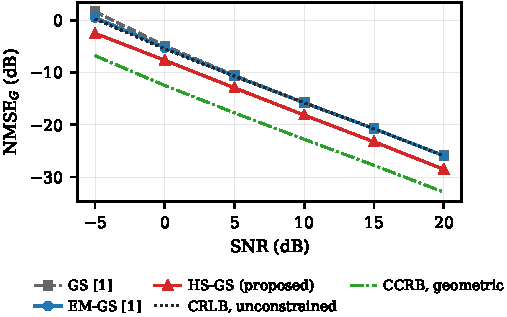
\includegraphics[width=\columnwidth]{fig/fig1_nmse_vs_snr.pdf}
\caption{NMSE versus SNR, bound-comparison configuration ($N=32$, $P=30$,
RSR $12$~dB, $T=50$, 4 Cadzow sweeps, ratio-of-sums). EM-GS tracks the
rank-one unconstrained CRLB closely at high SNR. Neither bound governs a
biased estimator.}
\label{fig:snr}
\end{figure}

\subsection{Aperture scaling}
\label{sec:aperture}

Fig.~\ref{fig:scaling} isolates the scaling. Averaged over the seven SNR
operating points at each array size the gain is
% src: trackB_hankel_emgs/results/experiment_B_array_size.csv (mean_gain_db,
% win_rate, active_frac); 4200/2800/1400 trials at N=8/16/32
$+0.029$, $+0.812$, $+2.452$~dB at $N=8,16,32$, with win rates $33.4$, $78.0$,
$96.3\%$ and the constraint active in $54.1$, $92.7$, $99.4\%$ of trials.
\textbf{Under the same averaging EM-GS varies by $0.036$~dB}, exactly as the
block-diagonal Fisher structure of \S\ref{sec:crlb} requires: the
$N$-dependence belongs to the structural prior, not to a degrading baseline.

$N=8$ is a mixed result, not a small positive one. There $\rmax=4$ while
$L_k\in\{3,\dots,7\}$, so the projection is inactive in $46\%$ of trials and
where active often truncates real components;
% src: trackB_hankel_emgs/results/experiment_A_snr.csv (N=8, P=30, 600
% trials per SNR point)
HS-GS gains $+0.744$~dB at
$-10$~dB SNR but loses $0.190$--$0.403$~dB above $0$~dB, and the sign of any
scalar summary depends on the pooling. Truncation bias does not shrink with
noise, so as variance falls the trade stops paying.

\begin{figure}[!t]
\centering
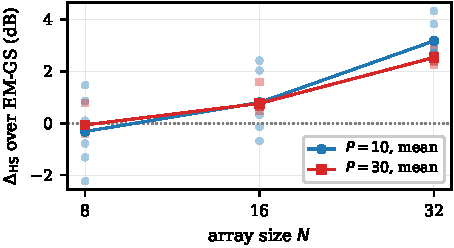
\includegraphics[width=\columnwidth]{fig/fig2_gain_vs_N.pdf}
\caption{Paired HS-GS gain over EM-GS versus array size, bound-comparison
configuration. Faint markers are the six individual SNR operating points,
solid lines their mean. At $N=8$ the points straddle zero, so no single scalar
summarises that array size.}
\label{fig:scaling}
\end{figure}

\subsection{From path count to effective rank}

Fixing $L_k=L$ across users and sweeping to the ceiling, the gain decays
strictly monotonically,
% src: trackB_hankel_emgs/results/experiment_C_path_count.csv
$7.04$, $3.56$, $1.79$, $1.04$, $0.58$, $0.27$, $0.05$, $-0.12$~dB for
$L=2,4,\dots,16$, with EM-GS flat to $0.19$~dB across the sweep --- which
rules out generic denoising, since that would persist at large $L$ where the
estimate is equally noisy rather than vanish exactly where the prior becomes
vacuous.

Re-indexing that sweep by $\reff/\rmax$ generalises it. The zero crossing moves
from $L/\rmax=0.90$ to
% src: reports/trackD_normalization.md A2
$\reff/\rmax=0.518$, and the useful region becomes $\reff/\rmax\lesssim0.5$ ---
a statement about any channel rather than about one simulator's $L$ values.
Fig.~\ref{fig:boundary} places $N\in\{16,32,64\}$ on that axis. The crossing is
% src: reports/trackD_partB9_analysis.json B1_collapse
$0.588$, $0.518$, $0.544$ across a fourfold change in aperture, a spread of
$0.070$; the $N=16$ and $N=64$ values are extrapolated from the last two
measured points rather than bracketed.

\textbf{The gain magnitude does not collapse onto the same axis, and we state
the residual rather than report a collapse.} Over the window both arrays
cover, $N=16$ lies above $N=64$ by a mean of $0.493$~dB and a maximum of
$0.901$~dB, one-signed throughout and monotone in $N$. We have no account of
it. One candidate is pencil quantisation at small capacity --- $\rmax(16)=8$
admits eight ranks against $32$ at $N=64$ --- but that is untested.

\begin{figure}[!t]
\centering
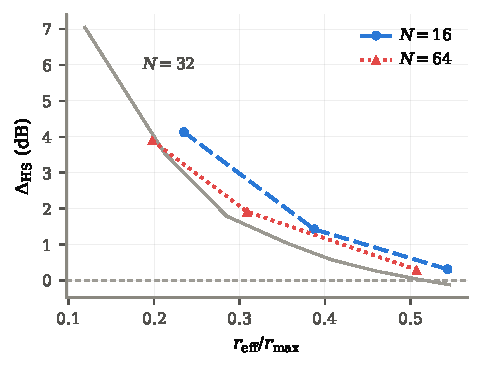
\includegraphics[width=\columnwidth]{fig/fig2_boundary_invariance.pdf}
\caption{$\dhs$ against $\reff/\rmax$, effective-rank configuration
(Table~\ref{tab:params}, right column; adaptive order, 1 Cadzow sweep, paired
median). The boundary is invariant to within $0.070$ across
$N\in\{16,32,64\}$; the magnitude is not, with a one-signed residual of mean
$0.493$~dB (max.\ $0.901$~dB).}
\label{fig:boundary}
\end{figure}

\subsection{Out-of-model prediction: the falsification test}
\label{sec:oom}

An earlier stage of this work concluded that robustness under clustered
propagation was not established and named the decisive next experiment:
\emph{repeat the principal comparison under a clustered generator --- a
falsification test, not a confirmation exercise.} This is that test, run twice.
In each case $\reff/\rmax$ was computed, a predicted $\dhs$ read off the
relation, and \textbf{the prediction committed to version control before the
measurement was run}; the relation was not refitted afterwards.

\textbf{Clustered Saleh--Valenzuela.} At $\reff/\rmax=0.331$ the relation
predicts $+1.30$~dB. Measured:
% src: reports/trackD_partB9_analysis.json B6_xiao.B6_xiao_clustered
$+1.173$~dB, CI $[+1.017,+1.380]$ --- an error of $0.13$~dB, prediction inside
the interval.

\textbf{A second, independently specified configuration.} We adopt the
receive-side Saleh--Valenzuela configuration of~\cite{precoding2408} --- $L=10$
paths, $\alpha_\ell\sim\CN(0,1)$, angles $\mathcal{U}(-90^\circ,90^\circ)$.~%
\todo{FILL IN AUTHORS of arXiv:2408.14366 from page 1 of the PDF; it is not
readable from the environment these results were produced in} That work is a
\emph{precoding} study, not a competing estimator, and only its channel
configuration is borrowed; it uses ULAs at both ends with incident and
departure angles, of which we use the receive side only. At
% src: reports/trackD_step0_cui_prediction.json and partB9_analysis.json
$\reff/\rmax=0.400$ the relation predicts $+0.648$~dB, interval
$[+0.367,+1.015]$. Measured: $+0.963$~dB, CI $[+0.808,+1.086]$. Inside the
registered interval and on the correct side of zero, but the point estimate is
$0.315$~dB low --- a larger error than the first, and we report it as such
rather than as a second $0.13$~dB hit. Together the two bound what the relation
is good for: it places an unseen channel on the correct part of the curve, and
it is not accurate to a tenth of a decibel in general.

\textbf{Clustering did not eliminate the gain}, which was the outcome the
earlier stage identified as possible. On a third reading in which all $40$ rays
are drawn independently, $\reff/\rmax$ rises to $0.748$, the relation predicts
$-0.12$~dB, and the measured median is exactly $0.000$~dB. The magnitude is
right to $0.12$~dB but \emph{the mechanism is not the predicted one}: rather
than degrading, the order-selection rule declines to project at all in
$29.1\%$ of trials against $1.4\%$ on the clustered model, without being told
which channel it faces. We report that as a partial match.

\begin{figure}[!t]
\centering
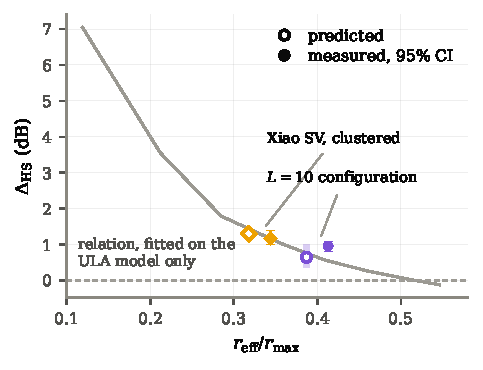
\includegraphics[width=\columnwidth]{fig/fig3_out_of_model.pdf}
\caption{Predictions registered before measurement, against measurement,
effective-rank configuration. The relation is fitted on the geometric ULA
model of \eqref{eq:chan} only; neither channel was used to fit or tune it.}
\label{fig:oom}
\end{figure}

\subsection{Users, and a replication}

The $K$-invariance predicted by \eqref{eq:compress} holds at SNR $\ge5$~dB,
where $\dhs$ across $K\in\{2,3,4\}$ at fixed $P/2K$ spans
% src: reports/trackD_partB9_analysis.json B2_K_invariance
$0.095$~dB. Pooled over all SNR it does not: the spread is $0.294$~dB and
monotone in $K$, missing a pre-registered falsifier of $0.3$~dB by
$0.006$~dB, which we do not present as a pass. The pooled trend is driven by
bins below $0$~dB where each cell contributes about $45$ trials.

\textbf{The two configurations are a replication.} At $N=32$ the same contrast
measures $+2.452$~dB under the bound-comparison configuration and $+2.680$~dB
under the effective-rank one --- different code, different RSR, iteration
count, Cadzow sweep count and pooling rule, agreeing to $0.23$~dB.

\section{Limitations and Conclusion}

A sparse geometric ULA channel makes each column's Hankel lifting rank
deficient, and this can be enforced inside an exact biased phase-retrieval
iteration without linearising the magnitude observation or estimating any
angle. Because the Fisher information is block diagonal across receive
elements, the unstructured baselines are flat in array size and HS-GS alone
converts a larger aperture into lower normalised error: $+0.03\to+2.45$~dB as
$N$ goes $8\to32$ against $0.036$~dB of baseline movement. The governing
variable is effective rank relative to capacity, not path count, and that
relation predicted the gain on two channel models it was never fitted to ---
one to within $0.13$~dB, the other inside a registered interval but $0.32$~dB
off. Clustered propagation, identified earlier as the decisive falsification
test, did not eliminate the gain.

\textbf{Limitations.} All results are simulation only, with no measured
hardware and no recorded channel data. They cover the geometric ULA model of
\eqref{eq:chan} and the Saleh--Valenzuela configurations of \S\ref{sec:oom},
and no claim is made beyond those families; the gain magnitude does not
collapse onto the proposed axis and its residual is unexplained; the benefit
is conditional and negative at $N=8$ above $0$~dB. A single scalar order is
imposed on all $K$ users despite their differing path counts, the projection
step is approximate on a non-convex set with no convergence guarantee, and
equal user power leaves near--far effects untested. Finally, both bounds
constrain unbiased estimators, and every estimator here is biased.

\bibliographystyle{IEEEtran}
\bibliography{refs}

\end{document}
